\chapter{TBD: Findings and Results}
For now, this chapter is a placeholder for the findings and results. Some were misplaced earlier in the thesis, others need to be written and then woven into the narrative.

\section{Findings}
\label{findings-section}

To Discuss:
\begin{itemize}
    \item Findings in the analytics
    \item Results in applying analytics
    \item Flaws in the analytics tools
    \item Results of using flawed analytics tools
    \item Software created to enable aspects of the research
    \item Results of the software we created for the research
\end{itemize}

The application of mobile analytics has enabled each of the development teams who participated in the research to materially improve their measured reliability. 

For the first case study the reliability was improved approximately 12x for the main Kiwix Android application by applying the approach identified in this research. 
During the initial improvement stages the reliability of the project's custom apps did not improve. These custom apps are built using the main application's source code, and when the improved codebase was used to create new releases of the custom apps their reliability also improved several fold.

\begin{figure}[htbp!]
    \centering
    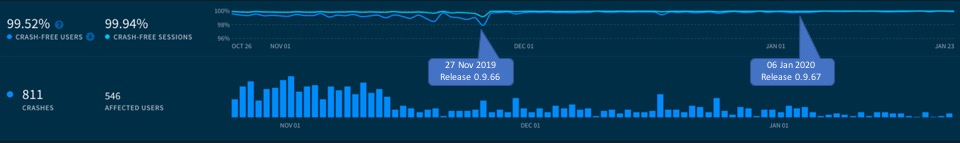
\includegraphics[width=\textwidth]{images/annotated_pocketcode_90_day_fabric_crashlytics_report.jpg}
    \caption{Pocket Code improvements in crash rate, in 90 days}
    %\Description{Pocket Code: When the project team investigated crashes they improved the reliability}
    \label{fig:pocketcode_improvements_in_crash_rate}
\end{figure}

An unacceptably high crash rate for the key Pocket Code Android app were tamed within two releases and 7 weeks by applying the approach described in this thesis. The changes needed to make the improvements were small. Figure \ref{fig:pocketcode_improvements_in_crash_rate} shows the improvement in crash rate as measured by Fabric Crashlytics. When the experiment started the crash rate was nearly four times the maximum threshold recommended by Google in their Android Vitals service and the project team had not been able to address the crash rate despite applying many of the recognised and recommended software development practices over several years~\cite{adamsen2015systematic_catrobat, luhana2018streamlining, ali2019behavior_catrobat, ali2019using_catrobat, hirsch2019approach_catrobat, schranz2019contributors_catrobat, slany2014tinkering}.

The developers continue to actively use mobile analytics to highlight potential quality issues and address pertinent issues promptly. One of the project teams chose to add an additional analytics tool to both their Android and iOS apps with the objective of improving the teams understanding of broader quality concerns. These quality concerns now also include usability. The team aims to use the data to improve the usability and user experience for their current and future users. They are designing the analytics to retain and protect user privacy, both important and highly relevant concerns.

Mobile Analytics can be incorporated as additional sources of information for development teams in harmony with other sources of information - it is not exclusive or exhaustive.

The analytics tools Google provides to developers of Android apps in Google Play Console have value despite the many flaws my research uncovered in their tools and reports. Some are mentioned in published papers~\cite{harty_google_play_console_insightful_development_using_android_vitals_and_pre_launch_reports, harty_better_android_apps_using_android_vitals, harty_improving_app_quality_despite_flawed_mobile_analytics}, the current known set are in this thesis. The research identified major differences in the reports and analytics provided by two analytics tools from the same company. There were both internal and cross-tool flaws and inconsistencies. Some of these have already been reported to Google in preparation for a full report to be submitted on completion of some ongoing research.

Fully automated pre-launch reports are effective at finding some quality flaws in Android apps at no financial cost and minimal effort by the app developers. These reports are provided by the app store and intended to help developers identify quality issues with their Android apps in order to address these issues so they do not affect end-users.


Google Play uses data collected automatically from users opted-in to provide usage and diagnostics data to Google. The data is collected at a per-device level, which means that one device could potentially report data from several user accounts, conversely for users who use multiple devices some may provide the data while others do not.